
\documentclass[draft]{agujournal2019}

\usepackage{url} 
\usepackage{lineno}
\usepackage[inline]{trackchanges} 
\usepackage{soul}
\usepackage{natbib}
\usepackage{float}

%\draftfalse

\journalname{AGU Advances}

%% Possible journal
%%% JGR oceans?


%%%%%%%%%%%%%%%%%%%%%%%%%%%%%%%%%%%

%% MACROS
\newcommand{\MKE}{\overline{\textrm{KE}}}
\newcommand{\KE}{\textrm{KE}}
\newcommand{\MEKE}{\overline{\textrm{EKE}}}
\newcommand{\EKE}{\textrm{EKE}}
\newcommand{\MCEKE}{\overline{\textrm{CEKE}}}
\newcommand{\CEKE}{\textrm{CEKE}}
\newcommand{\MREKE}{\overline{\textrm{REKE}}}
\newcommand{\REKE}{\textrm{REKE}}
\newcommand{\SST}{\textrm{SST}}
\newcommand{\SSH}{\textrm{SSH}}

\begin{document}
\title{Kinetic energy climatology of anisotropic oceanic features}

\authors{Josu\'e Mart\'inez-Moreno\affil{1}, Andrew McC. Hogg\affil{1}, and Matthew England\affil{2}}
\affiliation{1}{Research School of Earth Science and ARC Center of Excellence for Climate Extremes, Australian National University, Canberra, Australia}
\affiliation{2}{Climate Change Research Centre (CCRC), UNSW Australia, Sydney NSW, Australia}


\correspondingauthor{Josu\'e Mart\'inez-Moreno}{josue.martinezmoreno@anu.edu.au}


\begin{keypoints}
	\item Kinetic energy climatology reveals a surprising heterogeneity in the global ocean.
	\item Transient kinetic energy show significant increasing trends over large areas of the Southern Ocean and the Northern Hemisphere.
	\item Regional kinetic energy climatology strongly depends to the region dominant oceanic process.
\end{keypoints}


\begin{abstract}
	
	Ocean currents 

	\noindent\textbf{Plain summary}
	
\end{abstract}	
	
\section{Introduction}

Ocean currents are highly anisotropic and include coherent vortices and meandering jets. While coherent vortices (recirculating currents) are approximated as ellipses with axes smaller than the Rossby radius of deformation ($R_D$), meandering jets are narrow but elongated currents. The anisotropic nature of these features translates in ...


% %	Oceans are fundamental in the regulation of the climate system, as they have the capacity to absorb and transport heat, carbon, and other tracers through diverse flow scales which range from planetary (thermohaline circulation) to microscopic scales (turbulence). Mesoscale processes (hundreds of kilometres in scale) explain most of the temporal variability of kinetic energy (KE) and transport of tracers in the oceans. KE associated with mesoscale variability is commonly used as a diagnostic of the ocean state from satellite observations and numerical simulations.  
% %	
% %	Mean KE indicates regions in the ocean with persistent large scale circulation \citep{}, while the temporal variability of the KE field are directly linked to many transitory process in the ocean: coherent vortices, meanders, and waves. Transient events are strongly dependent to surface forcing and mixed layer variability \citep{}. 
% %	
% %	The transient component of the variability includes seasonal, inter-annual, and decadal variability \citep{}. 
% %	
% %	It has been reported an significant increase of the eddy kinetic energy (EKE) in the Southern Ocean \citep{}, 
% %	
% %	
% %	Add something here
% %	however the spatial variability is still unknown. 
% %	
% %	Despite satellite observations being coarser than 0.25$^\circ$ in many areas of the ocean, and a lack of studies exploring the global KE climatology, the present study will expands the understanding on surface ocean variability, and it is crucial  for ocean modeling community not only for ocean model validation, but also to  improve the eddy parametrization. 
% %	
% %	This study differs to \citet{Kang_On_2017} as we compute global climatologic focusing in the spatial distribution instead of the purely seasonality cycle.  The main goal of the present work is to generate a global climatology from the latest satellite observation dataset available, in order to complement the known information of the variability of the superficial Kinetic Energy.
% %	
% %	The data sources and methodology are described in section \ref{sec:Methods}. Global seasonality, inter-annual variability and trends are explored in sections \ref{sec:R_season},  \ref{sec:R_variability}, and  \ref{sec:R_trends} respectively. In section \ref{sec:R_regional} we present 3 regions in which we further investigate the temporal variability of kinetic energy and each of its components.
% %	
	\section{Methods}
	\label{sec:Methods}
% %	
% %	We compute global climatological montly KE, EKE, TEKE and TRKE by processing satellite observations and implementing TrackEddy an coherent eddy identification-reconstruction algorithm, with the capability to separate the Kinetic Energy from coherent and non-coherent features. The present study expands our understanding in the seasonal cycle, inter-annual variability and decadal trends.
% %	
% %	
% %	\subsection{Kinetic Energy decomposition}
% %	
% 	Kinetic energy is commonly divided into the mean and temporal variability components through a Reynolds decomposition. At a given time, the velocity field ($\mathbf{u}$) is split into the time mean ($\mathbf{\overline{u}}$) and time varying components ($\mathbf{u'}$). Additionally, as part of the climatology we also further decompose the eddy kinetic energy into the eddy kinetic energy contained by coherent features ($\mathbf{u'_e}$) and non-coherent ($\mathbf{u'_r}$). Therefore the KE equation can be written as:
	
% 	\begin{equation}
% 		\mathrm{KE}= \mathbf{\overline{u}}^2 +\underbrace{ \mathbf{u'_e}^2+ \mathbf{u'_r}^2 + \mathcal{O}^2}_{\mathbf{u'}^2}
% 	\end{equation}
	
% 	The second order terms ($\mathcal{O}$) are negligible as their time average is two orders of magnitude smaller than any other term. For more information about the decomposition of the field into coherent features and non-coherent features refer to \citet{Martinez_Kinetic_2019}.
% %	
% %	Qualitatively KE seasonality is similar to TKE and therefore we will focus mostly on the seasonality of TKE.
	\section{Results}
	\label{sec:Results}
	
	\subsection{Climatology}
	\label{subsec:R_season}
	
	\begin{figure}
	    \centering
	    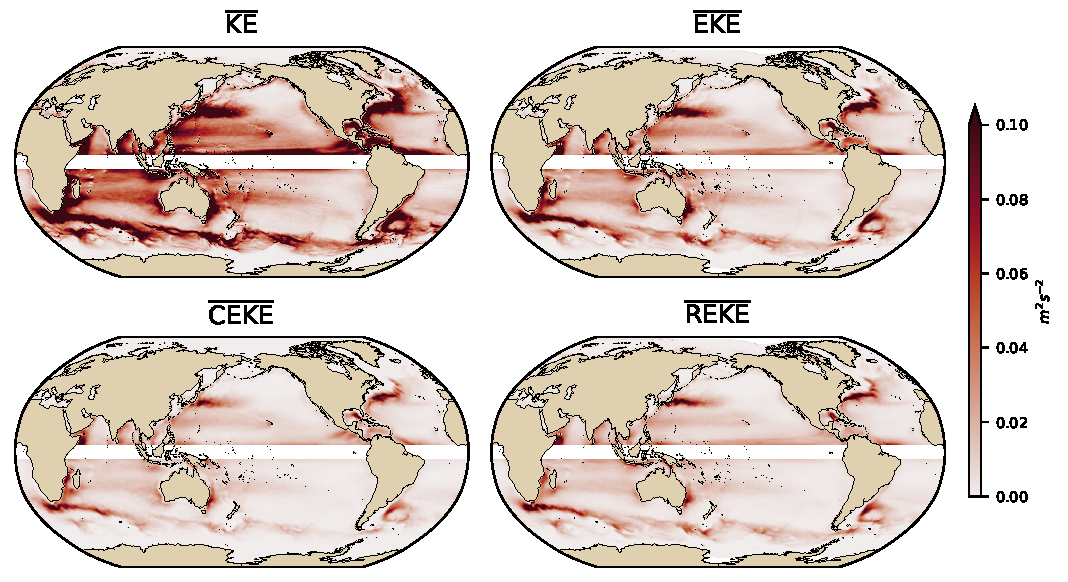
\includegraphics[width=1\textwidth]{figures/mean_ke_maps.pdf}
	    \caption{Caption}
	    \label{fig:my_label}
	\end{figure}
	
	\begin{itemize}
		\item Figure 1 shows regions with high values of Kinetic Energy at the Western Boundary Currents, ACC, and ocean gyres. 
		\item $\MEKE$ Explains $~70\%$ of $\MKE$, while $\MCEKE$ is $~40\%$ of $\MEKE$ and $\MREKE$  is $~60\%$ of $\MEKE$ 
		\item Maps show that $\MKE$, $\MEKE$, $\MCEKE$, and $\MREKE$ are dominated by the western boundary currents, the Antarctic Circumpolar Current (ACC).
	\end{itemize}
	
	\begin{figure}
	    \centering
	    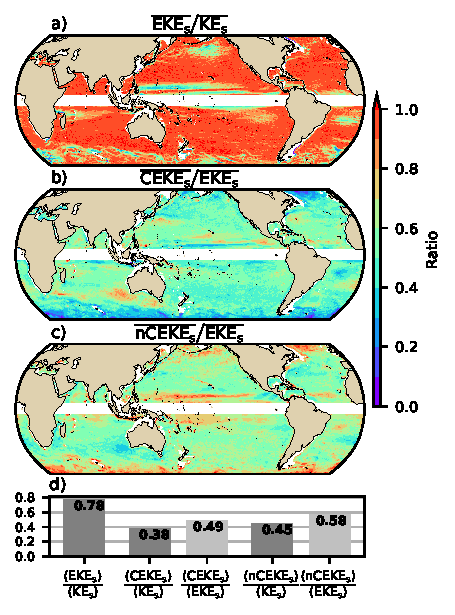
\includegraphics[width=1\textwidth]{figures/eke_ratio_map_all.pdf}
	    \caption{Ratios of the kinetic energy components. a) }
	    \label{fig:my_label}
	\end{figure}
	
    \begin{itemize}
		\item 
	\end{itemize}
	

	\begin{figure}
	    \centering
	    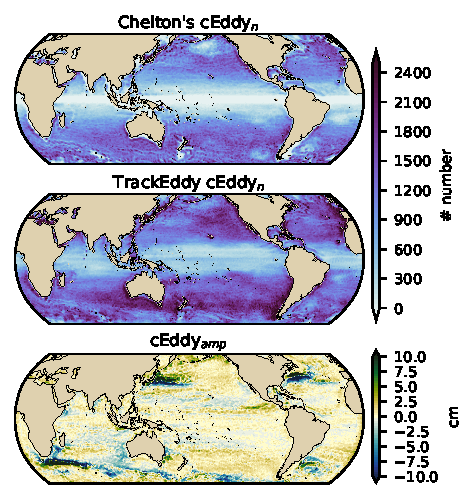
\includegraphics[width=1\textwidth]{figures/global_stats.pdf}
	    \caption{Ratios of the kinetic energy components. a) }
	    \label{fig:my_label}
	\end{figure}


	\begin{figure}
	    \centering
	    \includegraphics[width=1\textwidth]{figures/regional_eke_ceke_stats.pdf}
	    \caption{Climatology of regional statistics of the eddy field and coherent eddy field for the East Indian Ocean, East Tropical Pacific Ocean and South Atlantic Ocean. a-c Zoom to ratio of CEKE and EKE; d-f  mean eddy kinetic energy ($\MEKE$); g-i mean coherent eddy kinetic energy ($\MCEKE$); j-k count of identified coherent eddies between 1993-2019; and l-n mean coherent eddy amplitude between 1993-2019.}
	    \label{fig:my_label}
	\end{figure}

	

	\subsection{Seasonality}
	\label{subsec:R_season}
	

	\begin{figure}
	    \centering
	    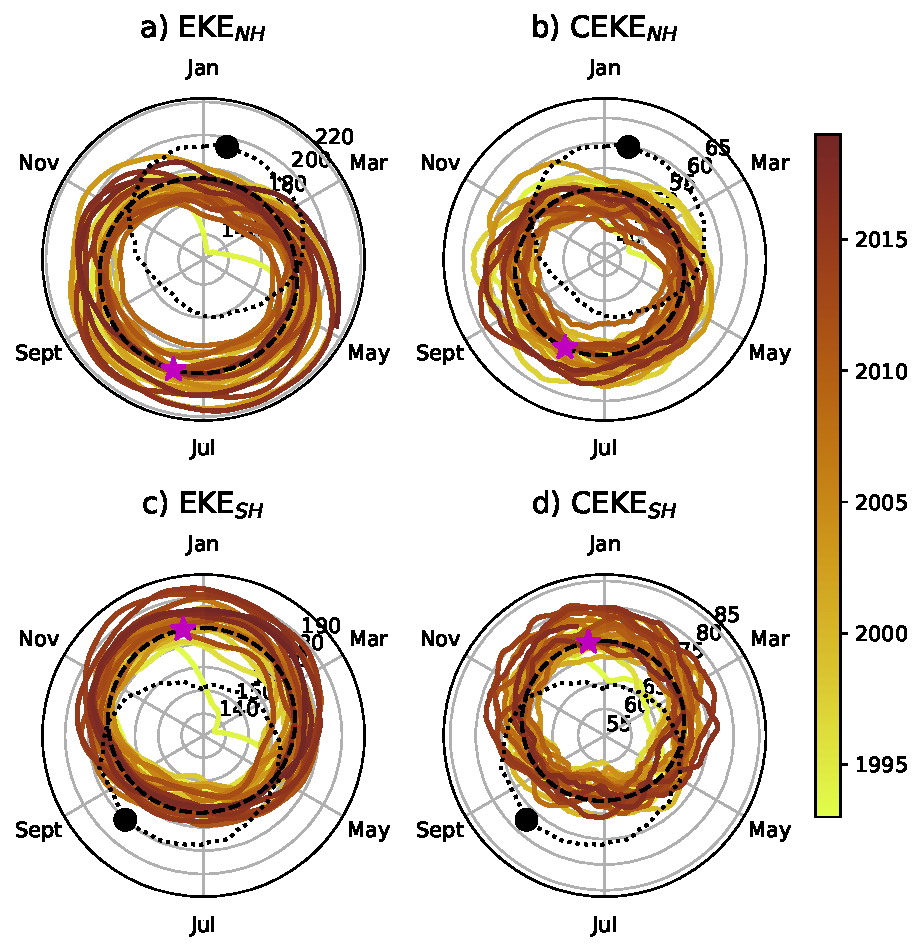
\includegraphics[width=1\textwidth]{figures/All_polar_plots.pdf}
	    \caption{Dashed lines correspond to the seasonal climatology of the fields. Dotted lines show the climatology of the wind magnitude. The green and magenta stars show the maximum of the seasonal cycle for the kinetic energy components and the wind magnitude, respectively. }
	    \label{fig:my_label}
	\end{figure}


% 	\begin{itemize}
% 		\item Western boundary currents show a strong seasonal patter, for example, the Kuroshio current maximum deviation from the mean occurs during the June-July-August (Northern Hemisphere (NH) summer), and lowest value during NH winter. Meanwhile, the Agulhas current at the Southern Hemisphere (SH) shows the opposite peak in the KE fields. This described phenomenology is similar to other western boundary currents.
% 		\item Gyres like the North Pacific Gyre (NPG), South Pacific Gyre (SPG), Indian Ocean Gyre (IOG) present a strong seasonal cycle. 
% 		\item The East Australian Current and the Leeuwin Current, Somali Current and East Indian Current show an intriguing dipole.
% 		\item The proposed TKE decomposition explains most of the regions in the ocean as a conjunction of Coherent processes (TEKE) and Non-coherent processes (TRKE). However, the Gulf of Tehuantepec (Mexico) shows that coherent processes dominate the regional TKE, as a direct response to the seasonal winds of the region (also shown in Fig. \ref{fig:tke_max_amp}). 
% 	\end{itemize}

% 	\begin{figure}[H]
% 		\centering
% 		\includegraphics[width=1\textwidth]{./figures/TKE_TEKE_seasonal_average_hc.pdf}
% 		\caption{Seasonal eddy kinetic energy (a,c,e,g) and transient eddy kinetic energy (b,d,f,h) from the AVISO+ dataset. DJF, JJA, MAM, and SON corresponds to the four seasons, respectively, December-January-February, March-April-May, June-July-August, and September-October-November}
% 		\label{fig:seasonal_global}
% 	\end{figure}
	
% 	\begin{itemize}
% 		\item NH and SH ${\mathrm{TKE}}$, ${\mathrm{TEKE}}$, and ${\mathrm{TRKE}}$ show a clear seasonal cycle as the monthly means are not concentric to center.
% 		\item NH shows large values of ${\mathrm{TKE}}$, ${\mathrm{TEKE}}$, and ${\mathrm{TRKE}}$ during June-July, while the SH is intensified between January-February (i.e. Summer for both hemispheres).
% 		\item NH shows an overlay between the years of the record, meaning that the observed variability is intrinsic to the system, however the SH shows an increase for the monthly average since the beginning of the record. In other words, early years in the record have smaller magnitudes over the year than the recent years. 
% 		\item The progressive intensification of the ${\mathrm{TKE}}$, ${\mathrm{TEKE}}$, and ${\mathrm{TRKE}}$ magnitude suggest an increase in the seasonal amplitude and increasing trends in the SH [Consistent with \citet{Hogg_Recent_2015} and \citet{Martinez_Kinetic_2019}].
% 		\item ${\mathrm{TEKE}}$ is highly variable within a year cycle, and it also show a the strongest seasonal dependence as the monthly means are shifted further towards summer in both hemispheres.
		
		
% 	\end{itemize}
	
	
% 	\begin{figure}[H]
% 		\centering
% 		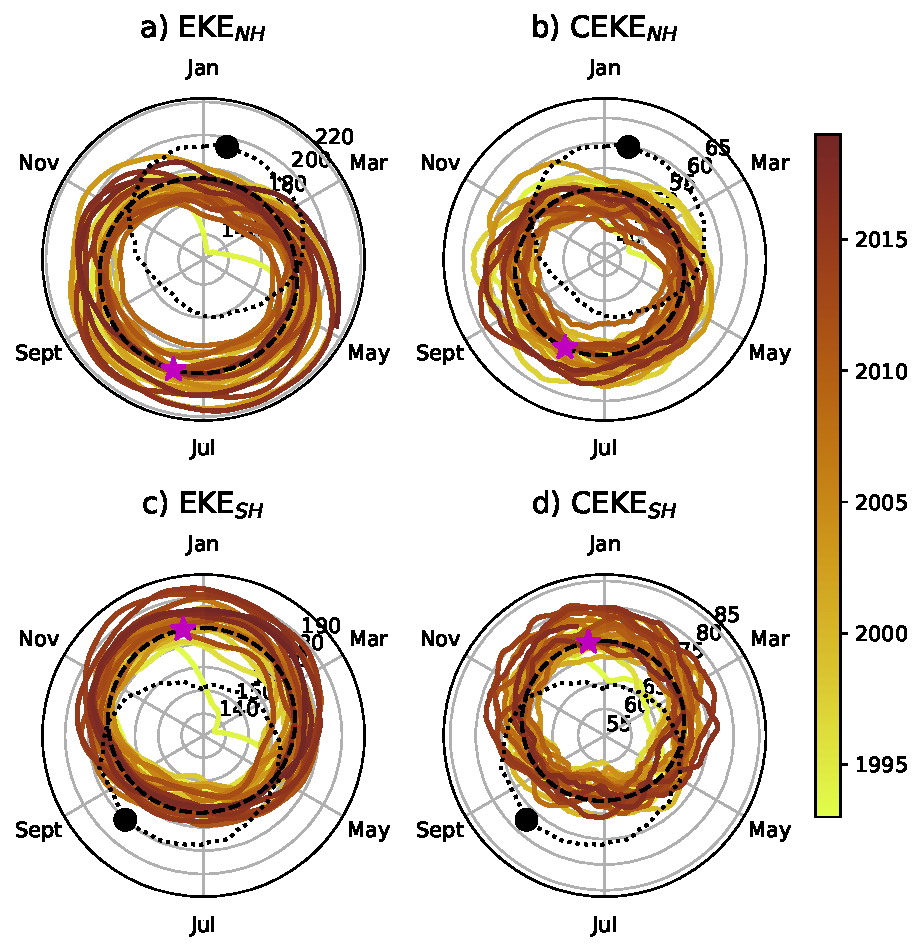
\includegraphics[width=1\textwidth]{./figures/All_polar_plots.pdf}
% 		\caption{Polar plot for monthly means from 1993 to 2017 a-b) transient kinetic energy, c-d) transient eddy kinetic energy, and e-f) transient residual kinetic for the northern hemisphere 10-60$^\circ$N (left column) and the southern hemisphere 10-60$^\circ$S (right column) from the AVISO+ dataset.}
% 		\label{fig:polar_seasonal}
% 	\end{figure}

% 	\begin{itemize}
% 		\item Histograms show a bi-modal distribution, attributed to XXX?
% 		\item NH summer has more frequent strong ${\mathrm{TKE}}$, ${\mathrm{TEKE}}$, and ${\mathrm{TRKE}}$ values than winter ( right tail of distribution).
% 		\item Lower tale in the NH presents a higher frequency. \textbf{Do you have any hypothesis for this?}
% 		\item The SH PDF has frequent larger magnitudes of ${\mathrm{TKE}}$, ${\mathrm{TEKE}}$, and ${\mathrm{TRKE}}$ during summer, than winter.
% 		\item I think there could be more interesting descriptions for this plot. I will like to discuss it in more detail with you. 
% 	\end{itemize}

% 	\begin{figure}[H]
% 		\centering
% 		\includegraphics[width=1\textwidth]{./figures/All_PDF_plots_log.pdf}
% 		\caption{PDF of the natural logarithm of the monthly satellite climatology of  a-b) transient kinetic energy, c-d) transient eddy kinetic energy, and e-f) transient residual kinetic energy for the northern hemisphere (left column) and the southern hemisphere (right column) from the AVISO+ dataset.} 
% 		\label{fig:pdf_seasonal}
% 	\end{figure}

% 	\begin{itemize}
% 		\item First EOF mode explain the seasonal cycle (variance $> 10\%$).
% 		\item There is a significant drop in the explained variance of the following modes (half of the explained variance of M$_1$).
% 		\item \textbf{I personally thing this is an important plot to explain why we are showing only the first mode in the following plot. However, I'm not sure what else to describe or if I should only state the first to points within the text. Do you have any particular suggestion?}
% 		\item \textbf{An interesting feature can be observed in M$_2$ between 2016-2018, it will be cool to further investigate why, however I think the best is to leave it outside the discussion.}
% 	\end{itemize}
	
% 	\begin{figure}[H]
% 		\centering
% 		\includegraphics[width=1\textwidth]{./figures/EOF_pcs_all.pdf}
% 		\caption{ a) EOF Mode 1 (M$_1$), b) EOF Mode 2 (M$_2$), and c) EOF Mode 3 (M$_3$) of eddy kinetic energy (black), transient eddy kinetic energy (green), and transient residual kinetic energy (yellow) from the AVISO+ dataset. d) Variance explained by each individual mode.}
% 		\label{fig:EOF_TKE}
% 	\end{figure}

% 	\begin{itemize}
% 		\item The regions with higher seasonal amplitude cycle correspond to the western boundary currents, oceanic gyres and regions of the ACC. 
% 		\item Perhaps we should merge this plot with the EOF plot (Fig. \ref{fig:EOF_TEKE}). \textbf{What do you think? }
% 	\end{itemize}
	
% 	\begin{figure}[H]
% 		\centering
% 		\includegraphics[width=0.9\textwidth]{./figures/All_monthly_max_amp.pdf}
% 		\caption{Month of maximum  a-b) transient kinetic energy, c-d) transient eddy kinetic energy, and e-f) transient residual kinetic energy from the AVISO+ dataset binned in $3^\circ\times3^\circ$ regions. Right panels b,d, and f shows the zonal averaged. Dots show regions where the maximum value is larger than six times the standard deviation ($6\sigma$)}
% 		\label{fig:tke_max_amp}
% 	\end{figure}
	
% 	\begin{itemize}
% 		\item Interesting dipoles at the east and wast coast of Australia, India and the equatorial pacific.\textbf{ I'm not sure which process could be producing this dipole or if it's an artifact from the EOF.}
% 		\item Western boundary currents show a clear seasonal cycle and the signs depends on the hemisphere.
% 		\item Most of the SO does not show a seasonal cycle except for key regions which could be attributed to topographic features.
% 	\end{itemize}
	
% 	\begin{figure}[H]
% 		\centering
% 		\includegraphics[width=0.9\textwidth]{./figures/EOF_all_montly_average.pdf}
% 		\caption{Mode 1 (EOF) for eddy kinetic energy (b), transient eddy kinetic energy (c), and transient residual kinetic energy}
% 		\label{fig:EOF_TEKE}
% 	\end{figure}
 	
% 	\begin{itemize}
% 		\item Month of maximum  ${\mathrm{TKE}}$, ${\mathrm{TEKE}}$, and ${\mathrm{TRKE}}$ presents a dominant month within the interiors of the ocean gyres. For example, NPG, NAG are present the largest values between May-July, while the SPG, SIG and SAG are large during November-January. 
% 		\item Contra-intuitively the ACC does not present a seasonal cycle, possible due to its high intrinsic variability or to small regions with large seasonal cycle shown in Fig.\ref{fig:tke_max_amp}. 
% 	\end{itemize}
% 	% Andrew contribution here.
% 	\begin{figure}[H]
% 		\centering
% 		\includegraphics[width=0.9\textwidth]{./figures/All_monthly_max_phase_sl_sat_05.pdf}
% 		\caption{Month of maximum  a-b) transient kinetic energy, c-d) transient eddy kinetic energy, and e-f) transient residual kinetic energy from the AVISO+ dataset binned in $3^\circ\times3^\circ$ regions. %Right panels b,d, and f shows the zonal averaged. 
% 		Dots show regions where the maximum value is larger than six times the standard deviation ($6\sigma$). Black solid and dashed lines show the 1~m and 0.5~m contour respectively, computed from the sea surface height mean climatology ($\overline{\mathrm{SSH}}$).}
% 		%of the barotropic stream function from a global 1$^\circ$ simulation (REF COSSIMA) To do: Test the $\overline{SSH}$ gyre contour definition.}
% 		\label{fig:tke_month}
% 	\end{figure}

%   	\subsection{Variability}
% 	\label{subsec:R_variability}
	
% 	\begin{itemize}
% 		\item SO shows clusters with correlation values with the SAM index above $0.4$. 
% 		\item The spare points in which the NH shows a correlation could be attributed to the known teleconnection between SAM and PDO.
% 		\item \textbf{Do you know why the tropics show an anti-correlation, I've look for papers about this, but I haven't find any.}
% 	\end{itemize}
	
% 	\begin{figure}[H]
% 		\centering
% 		\includegraphics[width=0.9\textwidth]{./figures/corr_SAM_ALL_KE.pdf}
% 		\caption{Lagged correlation between a) transient kinetic energy, b) transient eddy kinetic energy, and c) transient residual kinetic energy and the SAM index. Dots show regions where the highest correlation lag is larger than 36 months.}
% 		\label{fig:sam_corr}
% 	\end{figure}

% 	\begin{itemize}
% 		\item Correlation between ENSO and  ${\mathrm{TKE}}$, ${\mathrm{TEKE}}$, and ${\mathrm{TRKE}}$ is larger than the correlation with SAM.
% 		\item \textbf{Is the anti-correlation at the ACC a consequence of a tele-connection with SAM?}
% 		\item ENSO is highly correlated in the tropics. 
% 		\item\textbf{Interesting anti-correlation in the West Australian Current.}
% 	\end{itemize}
	
% 	\begin{figure}[H]
% 		\centering
% 		\includegraphics[width=0.9\textwidth]{./figures/corr_ENSO_ALL_KE_09.pdf}
% 		\caption{Lagged correlation between a) transient kinetic energy, b) transient eddy kinetic energy, and c) transient residual kinetic energy and ENSO. Dots show regions where the highest correlation lag is larger than 36 months.}
% 		\label{fig:enso_corr}
% 	\end{figure}
		
% 	\subsection{Trends}
% 	\label{subsec:R_trends}
	
% 	\begin{itemize}
% 		\item Regions with increasing trends are significant over 95\%. Note that most of the SO shows increasing trends. It's still unknown the consequences of the intensification of the kinetic energy field, further research is required. 
% 		\item NH western boundary currents ${\mathrm{TKE}}$, ${\mathrm{TEKE}}$, and ${\mathrm{TRKE}}$ pole-wards. This could be attributed to their pole-wards shift. 
% 		\item Decreasing trends are insignificant over the current dataset record and are mostly located in the NH.
% 		\item Increasing trends in  ${\mathrm{TKE}}$ are a combination of the trends in ${\mathrm{TEKE}}$, and ${\mathrm{TRKE}}$.
% 		\item Particularly increasing trends can be found near Australia. The highest trend in the record is found near the Tasman Front. This is attributed to an intensification of the coherent eddy fiend that in this particular region has a larger trend than the residual field. This could be an effect of the strengthening of the coherent eddy generation from the East Australian Current. Further investigation is required. 
% 	\end{itemize}

% % 	\begin{figure}[H]
% % 		\centering
% % 		\includegraphics[width=0.9\textwidth]{./figures/global_trend_all.pdf}
% % 		\caption{Global trends of a) transient kinetic energy, b)transient eddy kinetic energy, and c) transient residual kinetic energy from satellite observations between 1993-2018 binned in $6^\circ\times6^\circ$ degrees. Dots show regions where the trends are not significant according to the Pearson coefficient.}
% % 		\label{fig:trends_global}
% % 	\end{figure}

	
	\section{Summary and Conclusions}	
	
	\acknowledgments
	
	
	% Changes on document
	
	%%%%%%%%%%%%%%%%%%%%%%%%%%%%%%%%%%%%%%%%%%%%%%%%%%%%%%%%%%%%%%%%%%%%%
	% Track Changes:
	% To add words, \added{<word added>}
	% To delete words, \deleted{<word deleted>}
	% To replace words, \replaced{<word to be replaced>}{<replacement word>}
	% To explain why change was made: \explain{<explanation>} This will put
	% a comment into the right margin.
	
	%%%%%%%%%%%%%%%%%%%%%%%%%%%%%%%%%%%%%%%%%%%%%%%%%%%%%%%%%%%%%%%%%%%%%
	% At the end of the document, use \listofchanges, which will list the
	% changes and the page and line number where the change was made.
	
	% When final version, \listofchanges will not produce anything,
	% \added{<word or words>} word will be printed, \deleted{<word or words} will take away the word,
	% \replaced{<delete this word>}{<replace with this word>} will print only the replacement word.
	%  In the final version, \explain will not print anything.
	%%%%%%%%%%%%%%%%%%%%%%%%%%%%%%%%%%%%%%%%%%%%%%%%%%%%%%%%%%%%%%%%%%%%%
	
	%%%
%	\listofchanges
	%%%
	
	\bibliography{biblio.bib}
	
\end{document}
